% Options for packages loaded elsewhere
\PassOptionsToPackage{unicode}{hyperref}
\PassOptionsToPackage{hyphens}{url}
\PassOptionsToPackage{dvipsnames,svgnames*,x11names*}{xcolor}
%
\documentclass[
  10pt,
]{article}
\usepackage{lmodern}
\usepackage{setspace}
\usepackage{amssymb,amsmath}
\usepackage{ifxetex,ifluatex}
\ifnum 0\ifxetex 1\fi\ifluatex 1\fi=0 % if pdftex
  \usepackage[T1]{fontenc}
  \usepackage[utf8]{inputenc}
  \usepackage{textcomp} % provide euro and other symbols
\else % if luatex or xetex
  \usepackage{unicode-math}
  \defaultfontfeatures{Scale=MatchLowercase}
  \defaultfontfeatures[\rmfamily]{Ligatures=TeX,Scale=1}
  \setmainfont[]{DejaVu Serif}
  \setmonofont[]{DejaVu Sans Mono}
\fi
% Use upquote if available, for straight quotes in verbatim environments
\IfFileExists{upquote.sty}{\usepackage{upquote}}{}
\IfFileExists{microtype.sty}{% use microtype if available
  \usepackage[]{microtype}
  \UseMicrotypeSet[protrusion]{basicmath} % disable protrusion for tt fonts
}{}
\makeatletter
\@ifundefined{KOMAClassName}{% if non-KOMA class
  \IfFileExists{parskip.sty}{%
    \usepackage{parskip}
  }{% else
    \setlength{\parindent}{0pt}
    \setlength{\parskip}{6pt plus 2pt minus 1pt}}
}{% if KOMA class
  \KOMAoptions{parskip=half}}
\makeatother
\usepackage{xcolor}
\IfFileExists{xurl.sty}{\usepackage{xurl}}{} % add URL line breaks if available
\IfFileExists{bookmark.sty}{\usepackage{bookmark}}{\usepackage{hyperref}}
\hypersetup{
  colorlinks=true,
  linkcolor=red,
  filecolor=red,
  citecolor=red,
  urlcolor=red,
  pdfcreator={LaTeX via pandoc}}
\urlstyle{same} % disable monospaced font for URLs
\usepackage[margin=1cm,top=1cm,bottom=1cm,left=1cm,right=1cm,includeheadfoot]{geometry}
\usepackage{listings}
\newcommand{\passthrough}[1]{#1}
\lstset{defaultdialect=[5.3]Lua}
\lstset{defaultdialect=[x86masm]Assembler}
\usepackage{longtable,booktabs}
% Correct order of tables after \paragraph or \subparagraph
\usepackage{etoolbox}
\makeatletter
\patchcmd\longtable{\par}{\if@noskipsec\mbox{}\fi\par}{}{}
\makeatother
% Allow footnotes in longtable head/foot
\IfFileExists{footnotehyper.sty}{\usepackage{footnotehyper}}{\usepackage{footnote}}
\makesavenoteenv{longtable}
\usepackage{graphicx}
\makeatletter
\def\maxwidth{\ifdim\Gin@nat@width>\linewidth\linewidth\else\Gin@nat@width\fi}
\def\maxheight{\ifdim\Gin@nat@height>\textheight\textheight\else\Gin@nat@height\fi}
\makeatother
% Scale images if necessary, so that they will not overflow the page
% margins by default, and it is still possible to overwrite the defaults
% using explicit options in \includegraphics[width, height, ...]{}
\setkeys{Gin}{width=\maxwidth,height=\maxheight,keepaspectratio}
% Set default figure placement to htbp
\makeatletter
\def\fps@figure{htbp}
\makeatother
\setlength{\emergencystretch}{3em} % prevent overfull lines
\providecommand{\tightlist}{%
  \setlength{\itemsep}{0pt}\setlength{\parskip}{0pt}}
\setcounter{secnumdepth}{3}
% Enable graphics inclusion and ensure figure numbering works
\usepackage{graphicx}
\renewcommand{\figurename}{Figure}

% Configure fonts for Unicode support with fallbacks
\usepackage{newunicodechar}
\newunicodechar{⁴}{\textsuperscript{4}}
\newunicodechar{₄}{\textsubscript{4}}

% Enhanced code block styling for better contrast and readability
\usepackage{fancyvrb}
\usepackage{xcolor}
\usepackage{listings}

% Define custom colors for code blocks
\definecolor{codebg}{RGB}{245, 245, 245}      % Light gray background
\definecolor{codeborder}{RGB}{200, 200, 200}  % Medium gray border
\definecolor{codefg}{RGB}{50, 50, 50}         % Dark gray text

% Configure Verbatim environment for inline code
\DefineVerbatimEnvironment{Verbatim}{Verbatim}{%
    fontsize=\small,
    frame=single,
    framerule=0.5pt,
    framesep=3pt,
    rulecolor=\color{codeborder},
    bgcolor=\color{codebg},
    fgcolor=\color{codefg}
}

% Configure code block styling
\DefineVerbatimEnvironment{Highlighting}{Verbatim}{%
    fontsize=\footnotesize,
    frame=single,
    framerule=0.5pt,
    framesep=5pt,
    rulecolor=\color{codeborder},
    bgcolor=\color{codebg},
    fgcolor=\color{codefg}
}

% Style inline code with \texttt
\renewcommand{\texttt}[1]{%
    \colorbox{codebg}{\color{codefg}\ttfamily #1}%
}

% Configure listings package for code blocks
\lstset{
    backgroundcolor=\color{codebg},
    basicstyle=\footnotesize\ttfamily\color{codefg},
    breakatwhitespace=false,
    breaklines=true,
    captionpos=b,
    commentstyle=\color{codefg},
    deletekeywords={...},
    escapeinside={\%*}{*)},
    extendedchars=true,
    frame=single,
    framerule=0.5pt,
    framesep=5pt,
    keepspaces=true,
    keywordstyle=\color{codefg},
    language=Python,
    morekeywords={*,...},
    numbers=left,
    numbersep=5pt,
    numberstyle=\tiny\color{codefg},
    rulecolor=\color{codeborder},
    showspaces=false,
    showstringspaces=false,
    showtabs=false,
    stepnumber=1,
    stringstyle=\color{codefg},
    tabsize=2,
    title=\lstname
}

% Override any Pandoc default lstset configurations
\AtBeginDocument{
    \lstset{
        backgroundcolor=\color{codebg},
        basicstyle=\footnotesize\ttfamily\color{codefg},
        frame=single,
        framerule=0.5pt,
        framesep=5pt,
        rulecolor=\color{codeborder},
        numbers=left,
        numbersep=5pt,
        numberstyle=\tiny\color{codefg}
    }
}

% Configure hyperref colors consistently
\AtBeginDocument{
% Override pandoc's hidelinks setting with consistent options
\hypersetup{
    colorlinks=true,
    allcolors=red,
    linkcolor=red,
    urlcolor=red,
    citecolor=red,
    filecolor=red,
    menucolor=red,
    linktoc=all
}
}

% Simple page break support for document structure
% Note: Page breaks are handled in the markdown generation, not here

\title{Quadray Analytical Details and Methods}
\author{Daniel Ari Friedman\\ ORCID: 0000-0001-6232-9096\\ Email: daniel@activeinference.institute}
\date{August 15, 2025}

\begin{document}
\maketitle

{
\hypersetup{linkcolor=black}
\setcounter{tocdepth}{3}
\tableofcontents
}
\setstretch{1.0}
\hypertarget{quadray-analytical-details-and-methods}{%
\section{Quadray Analytical Details and
Methods}\label{quadray-analytical-details-and-methods}}

\hypertarget{overview}{%
\subsection{Overview}\label{overview}}

This section provides detailed analytical methods for working with
Quadray coordinates, including coordinate conventions, volume
calculations, and optimization approaches. We emphasize the distinction
between different 4D frameworks and provide practical computational
methods.

\hypertarget{coxeter.4d-euclidean-4d-geometry-and-regular-polytopes}{%
\subsection{Coxeter.4D: Euclidean 4D Geometry and Regular
Polytopes}\label{coxeter.4d-euclidean-4d-geometry-and-regular-polytopes}}

\begin{itemize}
\tightlist
\item
  \textbf{Coxeter groups}: finite reflection groups generated by
  reflections across hyperplanes with dihedral angles \(\pi/m_{ij}\).
  The Coxeter matrix \(M = (m_{ij})\) defines the group via relations
\end{itemize}

\begin{equation}\label{eq:coxeter_relations}
(s_i s_j)^{m_{ij}} = e,\quad m_{ii}=1,\; m_{ij}\in\{2,3,4,\ldots,\infty\}\,.
\end{equation}

\begin{itemize}
\tightlist
\item
  \textbf{Gram matrix and angles}: for a Coxeter system realized by unit
  normal vectors to reflection hyperplanes, the Gram matrix is
\end{itemize}

\begin{equation}\label{eq:coxeter_gram}
G_{ij} = \begin{cases}
1, & i=j \\
-\cos\!\left(\dfrac{\pi}{m_{ij}}\right), & i\ne j
\end{cases}
\end{equation}

\begin{itemize}
\tightlist
\item
  \textbf{4D regular polytopes and diagrams}: canonical finite Coxeter
  diagrams in 4D include:

  \begin{itemize}
  \tightlist
  \item
    \([3,3,3]\): symmetry of the 5-cell (pentachoron), the 4D simplex.
  \item
    \([4,3,3]\): symmetry of the 8-cell/16-cell pair
    (tesseract--cross-polytope).
  \item
    \([3,4,3]\): symmetry of the unique self-dual 24-cell. These
    diagrams compactly encode generating reflections and dihedral angles
    between mirrors, guiding constructions and projections of 4D
    polytopes. See references:
    \href{https://en.wikipedia.org/wiki/Regular_polytope}{Regular
    polytopes (Coxeter)} and
    \href{https://en.wikipedia.org/wiki/Coxeter_group}{Coxeter group};
    lattice context:
    \href{https://link.springer.com/book/10.1007/978-1-4757-6568-7}{Sphere
    Packings, Lattices and Groups}.
  \end{itemize}
\item
  \textbf{Bridge to our methods}: when we compute Euclidean volumes from
  edge lengths (e.g., Cayley--Menger; Eq. \eqref{eq:cayley_menger}), we
  are operating squarely in the Coxeter.4D/Euclidean paradigm,
  independent of Quadray unit conventions.
\end{itemize}

\hypertarget{einstein.4d-minkowski-spacetime-metric-and-field-equations}{%
\subsection{Einstein.4D (Minkowski spacetime): metric and field
equations}\label{einstein.4d-minkowski-spacetime-metric-and-field-equations}}

\begin{itemize}
\tightlist
\item
  \textbf{Metric}: an indefinite inner product space with line element
  (mostly-plus convention) given by
\end{itemize}

\begin{equation}\label{eq:einstein_line_element_methods}
ds^2 = -c^2\,dt^2 + dx^2 + dy^2 + dz^2
\end{equation}

The metric tensor is \(g_{\mu\nu}\).

\begin{itemize}
\tightlist
\item
  \textbf{Einstein field equations}: curvature responds to
  stress--energy per
\end{itemize}

\begin{equation}\label{eq:efe}
G_{\mu \nu} + \Lambda\, g_{\mu \nu} = \kappa\, T_{\mu \nu},\qquad \kappa = \frac{8\pi G}{c^4}\,.
\end{equation}

\begin{itemize}
\tightlist
\item
  \textbf{Einstein tensor}: defined from the Ricci tensor \(R_{\mu\nu}\)
  and scalar curvature \(R\) by
\end{itemize}

\begin{equation}\label{eq:einstein_tensor}
G_{\mu \nu} = R_{\mu \nu} - \tfrac{1}{2}\,R\, g_{\mu \nu},\qquad R = g^{\mu\nu} R_{\mu\nu}\,.
\end{equation}

\begin{itemize}
\tightlist
\item
  \textbf{Scope note}: we use Einstein.4D primarily as a metric/geodesic
  analogy when discussing information geometry (e.g., Fisher metric and
  natural gradient). Physical constants \(G,c,\Lambda\) do not appear in
  Quadray lattice methods and should not be mixed with IVM unit
  conventions. References:
  \href{https://en.wikipedia.org/wiki/Einstein_field_equations}{Einstein
  field equations},
  \href{https://en.wikipedia.org/wiki/Minkowski_space}{Minkowski space},
  \href{https://en.wikipedia.org/wiki/Fisher_information}{Fisher
  information}.
\end{itemize}

\hypertarget{fuller.4d-coordinates-and-normalization}{%
\subsection{Fuller.4D Coordinates and
Normalization}\label{fuller.4d-coordinates-and-normalization}}

\begin{itemize}
\tightlist
\item
  Quadray vector q = (a,b,c,d), a,b,c,d ≥ 0, with at least one
  coordinate zero under normalization.
\item
  Projective normalization can add/subtract (k,k,k,k) without changing
  direction; choose k to enforce non-negativity and one zero minimum.
\item
  Isotropic Vector Matrix (IVM): integer quadrays describe CCP sphere
  centers; the 12 permutations of \{2,1,1,0\} form the cuboctahedron
  (vector equilibrium).

  \begin{itemize}
  \tightlist
  \item
    Integer-coordinate models: assigning unit IVM tetravolume to the
    regular tetrahedron yields integer coordinates for several familiar
    polyhedra (inverse tetrahedron, cube, octahedron, rhombic
    dodecahedron, cuboctahedron) when expressed as linear combinations
    of the four quadray basis vectors. See overview:
    \href{https://en.wikipedia.org/wiki/Quadray_coordinates}{Quadray
    coordinates}.
  \end{itemize}
\end{itemize}

\hypertarget{conversions-and-vector-operations-quadray-cartesian-fuller.4d-coxeter.4dxyz}{%
\subsection{Conversions and Vector Operations: Quadray ↔ Cartesian
(Fuller.4D ↔
Coxeter.4D/XYZ)}\label{conversions-and-vector-operations-quadray-cartesian-fuller.4d-coxeter.4dxyz}}

\begin{itemize}
\tightlist
\item
  \textbf{Embedding conventions} determine the linear maps between
  Quadray (Fuller.4D) and Cartesian XYZ (a 3D slice or embedding aligned
  with Coxeter.4D conventions).
\item
  \textbf{References}: Urner provides practical conversion write-ups and
  matrices; see:

  \begin{itemize}
  \tightlist
  \item
    Quadrays and XYZ:
    \href{https://www.grunch.net/synergetics/quadxyz.html}{Urner --
    Quadrays and XYZ}
  \item
    Introduction with examples:
    \href{https://www.grunch.net/synergetics/quadintro.html}{Urner --
    Quadray intro}
  \end{itemize}
\item
  \textbf{Implementation}: choose a fixed tetrahedral embedding;
  construct a 3×4 matrix M that maps (a,b,c,d) to (x,y,z), respecting
  A,B,C,D directions to tetra vertices. The inverse map can be defined
  up to projective normalization (adding (k,k,k,k)). When comparing
  volumes, use the \passthrough{\lstinline!S3=\\sqrt\{9/8\}!} scale to
  convert XYZ (Euclidean) volumes to IVM (Fuller.4D) units.
\item
  \textbf{Vector view}: treat \passthrough{\lstinline!q!} as a vector
  with magnitude and direction; define dot products and norms by pushing
  to XYZ via \passthrough{\lstinline!M!}.
\end{itemize}

\hypertarget{integer-coordinate-constructions-compact-derivation-box}{%
\subsubsection{Integer-coordinate constructions (compact derivation
box)}\label{integer-coordinate-constructions-compact-derivation-box}}

\begin{itemize}
\tightlist
\item
  Under the synergetics convention (unit regular tetrahedron has
  tetravolume 1), many familiar solids admit Quadray integer
  coordinates. For example, the octahedron at the same edge length has
  tetravolume 4, and its vertices can be formed as integer linear
  combinations of the four axes A,B,C,D subject to the Quadray
  normalization rule.
\item
  The cuboctahedron (vector equilibrium) arises as the shell of the 12
  nearest IVM neighbors given by the permutations of \((2,1,1,0)\). The
  rhombic dodecahedron (tetravolume 6) is the Voronoi cell of the
  FCC/CCP packing centered at the origin under the same embedding.
\item
  See the following figure for a schematic summary of these
  relationships.
\end{itemize}

\begin{longtable}[]{@{}lll@{}}
\toprule
\begin{minipage}[b]{0.30\columnwidth}\raggedright
Object\strut
\end{minipage} & \begin{minipage}[b]{0.30\columnwidth}\raggedright
Quadray construction (sketch)\strut
\end{minipage} & \begin{minipage}[b]{0.30\columnwidth}\raggedright
IVM volume\strut
\end{minipage}\tabularnewline
\midrule
\endhead
\begin{minipage}[t]{0.30\columnwidth}\raggedright
Regular tetrahedron\strut
\end{minipage} & \begin{minipage}[t]{0.30\columnwidth}\raggedright
Vertices \passthrough{\lstinline!o=(0,0,0,0)!},
\passthrough{\lstinline!p=(2,1,0,1)!},
\passthrough{\lstinline!q=(2,1,1,0)!},
\passthrough{\lstinline!r=(2,0,1,1)!}\strut
\end{minipage} & \begin{minipage}[t]{0.30\columnwidth}\raggedright
1\strut
\end{minipage}\tabularnewline
\begin{minipage}[t]{0.30\columnwidth}\raggedright
Cube (same edge)\strut
\end{minipage} & \begin{minipage}[t]{0.30\columnwidth}\raggedright
Union of 3 mutually orthogonal rhombic belts wrapped on the tetra frame;
edges tracked by XYZ embedding; compare the following figure\strut
\end{minipage} & \begin{minipage}[t]{0.30\columnwidth}\raggedright
3\strut
\end{minipage}\tabularnewline
\begin{minipage}[t]{0.30\columnwidth}\raggedright
Octahedron (same edge)\strut
\end{minipage} & \begin{minipage}[t]{0.30\columnwidth}\raggedright
Convex hull of mid-edges of the tetra frame (pairwise axis sums
normalized)\strut
\end{minipage} & \begin{minipage}[t]{0.30\columnwidth}\raggedright
4\strut
\end{minipage}\tabularnewline
\begin{minipage}[t]{0.30\columnwidth}\raggedright
Rhombic dodecahedron\strut
\end{minipage} & \begin{minipage}[t]{0.30\columnwidth}\raggedright
Voronoi cell of FCC/CCP packing at origin (dual to cuboctahedron)\strut
\end{minipage} & \begin{minipage}[t]{0.30\columnwidth}\raggedright
6\strut
\end{minipage}\tabularnewline
\begin{minipage}[t]{0.30\columnwidth}\raggedright
Cuboctahedron (vector equilibrium)\strut
\end{minipage} & \begin{minipage}[t]{0.30\columnwidth}\raggedright
Shell of the 12 nearest IVM neighbors: permutations of
\passthrough{\lstinline!(2,1,1,0)!}\strut
\end{minipage} & \begin{minipage}[t]{0.30\columnwidth}\raggedright
20\strut
\end{minipage}\tabularnewline
\begin{minipage}[t]{0.30\columnwidth}\raggedright
Truncated octahedron\strut
\end{minipage} & \begin{minipage}[t]{0.30\columnwidth}\raggedright
Archimedean solid with 6 square and 8 hexagonal faces; space-filling
tiling\strut
\end{minipage} & \begin{minipage}[t]{0.30\columnwidth}\raggedright
20\strut
\end{minipage}\tabularnewline
\bottomrule
\end{longtable}

Small coordinate examples (subset):

\begin{itemize}
\tightlist
\item
  Cuboctahedron neighbors (representatives):
  \passthrough{\lstinline!(2,1,1,0)!},
  \passthrough{\lstinline!(2,1,0,1)!},
  \passthrough{\lstinline!(2,0,1,1)!},
  \passthrough{\lstinline!(1,2,1,0)!}; the full shell is all distinct
  permutations.
\item
  Tetrahedron:
  \passthrough{\lstinline![(0,0,0,0), (2,1,0,1), (2,1,1,0), (2,0,1,1)]!}.
\end{itemize}

Short scripts:

\begin{lstlisting}[language=bash]
python3 quadmath/scripts/polyhedra_quadray_constructions.py
\end{lstlisting}

Programmatic check (neighbors, equal radii, adjacency):

\begin{lstlisting}[language=Python]
import numpy as np
from examples import example_cuboctahedron_vertices_xyz

xyz = np.array(example_cuboctahedron_vertices_xyz())
r = np.linalg.norm(xyz[0])
assert np.allclose(np.linalg.norm(xyz, axis=1), r)

# Touching neighbors have separation 2r
touch = []
for i in range(len(xyz)):
    for j in range(i+1, len(xyz)):
        d = np.linalg.norm(xyz[i] - xyz[j])
        if abs(d - 2*r) / (2*r) < 0.05:
            touch.append((i, j))
assert len(touch) > 0
\end{lstlisting}

\hypertarget{example-vertex-lists-and-volume-checks-illustrative}{%
\subsubsection{Example vertex lists and volume checks
(illustrative)}\label{example-vertex-lists-and-volume-checks-illustrative}}

The following snippets use canonical IVM neighbor points (permutations
of \((2,1,1,0)\)) to illustrate simple decompositions consistent with
synergetics volumes. Each tetra volume is computed via
\passthrough{\lstinline!ace\_tetravolume\_5x5!} and summed.

Octahedron (V = 4) as four unit IVM tetras around the origin:

\begin{lstlisting}[language=Python]
from quadray import Quadray, ace_tetravolume_5x5

o = Quadray(0,0,0,0)
T = [
    (Quadray(2,1,0,1), Quadray(2,1,1,0), Quadray(2,0,1,1)),
    (Quadray(1,2,0,1), Quadray(1,2,1,0), Quadray(0,2,1,1)),
    (Quadray(1,1,2,0), Quadray(1,0,2,1), Quadray(0,1,2,1)),
    (Quadray(2,0,1,1), Quadray(1,2,0,1), Quadray(0,1,2,1)),  # representative variant
]
V_oct = sum(ace_tetravolume_5x5(o, a, b, c) for (a,b,c) in T)
\end{lstlisting}

Cube (V = 3) as three unit IVM tetras (orthant-like around the origin):

\begin{lstlisting}[language=Python]
from quadray import Quadray, ace_tetravolume_5x5

o = Quadray(0,0,0,0)
triples = [
    (Quadray(2,1,0,1), Quadray(2,1,1,0), Quadray(2,0,1,1)),
    (Quadray(1,2,0,1), Quadray(1,2,1,0), Quadray(0,2,1,1)),
    (Quadray(1,1,2,0), Quadray(1,0,2,1), Quadray(0,1,2,1)),
]
V_cube = sum(ace_tetravolume_5x5(o, a, b, c) for (a,b,c) in triples)
\end{lstlisting}

Notes.

\begin{itemize}
\tightlist
\item
  These decompositions are illustrative and use canonical IVM neighbor
  triples that produce unit tetras under
  \passthrough{\lstinline!ace\_tetravolume\_5x5!}. Other equivalent
  tilings are possible.
\item
  Volumes are invariant to adding \((k,k,k,k)\) to each vertex of a
  tetra (projective normalization), which the 5×5 determinant respects.
\end{itemize}

\hypertarget{sec:integer_volume}{%
\subsection{Integer Volume Quantization}\label{sec:integer_volume}}

For a tetrahedron with vertices P₀..P₃ in the Quadray integer lattice
(Fuller.4D):

\begin{equation}\label{eq:lattice_det}
V = \tfrac{1}{6}\,\left|\det\,[\,P_1 - P_0,\; P_2 - P_0,\; P_3 - P_0\,]\right|
\end{equation}

\begin{itemize}
\tightlist
\item
  With integer coordinates, the determinant is integer; lattice
  tetrahedra yield integer volumes.
\item
  Unit conventions: regular tetrahedron volume = 1 (synergetics).
\end{itemize}

Notes.

\begin{itemize}
\tightlist
\item
  \(P_0,\ldots,P_3\) are tetrahedron vertices in Quadray coordinates.
\item
  \(V\) is the Euclidean volume measured in IVM tetra-units; the \(1/6\)
  factor converts the parallelepiped determinant to a tetra volume.
\item
  Background and variations are discussed under Tetrahedron volume
  formulas:
  \href{https://en.wikipedia.org/wiki/Tetrahedron\#Volume}{Tetrahedron
  -- volume}.
\end{itemize}

Tom Ace 5×5 determinant (tetravolume directly from quadrays):

\begin{equation}\label{eq:ace5x5}
V_{ivm} = \tfrac{1}{4} \left| \det \begin{pmatrix}
 a_0 & a_1 & a_2 & a_3 & 1 \\
 b_0 & b_1 & b_2 & b_3 & 1 \\
 c_0 & c_1 & c_2 & c_3 & 1 \\
 d_0 & d_1 & d_2 & d_3 & 1 \\
 1 & 1 & 1 & 1 & 0
\end{pmatrix} \right|
\end{equation}

This returns the same integer volumes for lattice tetrahedra. See the
implementation \passthrough{\lstinline!ace\_tetravolume\_5x5!}.

Notes.

\begin{itemize}
\tightlist
\item
  Rows correspond to the Quadray 4-tuples of the four vertices with a
  final affine column of ones; the last row enforces projective
  normalization.
\item
  The factor \(\tfrac{1}{4}\) returns tetravolumes in IVM units
  consistent with synergetics. See also
  \href{https://en.wikipedia.org/wiki/Quadray_coordinates}{Quadray
  coordinates}.
\end{itemize}

Equivalently, define the 5×5 matrix of quadray coordinates augmented
with an affine 1 as

\begin{equation}\label{eq:ace5x5_expanded}
M(q_0,q_1,q_2,q_3) = \begin{bmatrix}
q_{01} & q_{02} & q_{03} & q_{04} & 1 \\
q_{11} & q_{12} & q_{13} & q_{14} & 1 \\
q_{21} & q_{22} & q_{23} & q_{24} & 1 \\
q_{31} & q_{32} & q_{33} & q_{34} & 1 \\
1 & 1 & 1 & 1 & 0
\end{bmatrix},\qquad V_{ivm} = \tfrac{1}{4}\,\big|\det M(q_0,q_1,q_2,q_3)\big|\,.
\end{equation}

Points vs vectors: subtracting points is shorthand for forming edge
vectors. We treat quadray 4-tuples as vectors from the origin;
differences like \((P_1-P_0)\) mean ``edge vectors,'' avoiding ambiguity
between ``points'' and ``vectors.''

Equivalently via Cayley--Menger determinant (Coxeter.4D/Euclidean
lengths)
(\href{https://en.wikipedia.org/wiki/Cayley\%E2\%80\%93Menger_determinant}{Cayley--Menger
determinant}):

\begin{equation}\label{eq:cayley_menger}
288\,V^2 = \det\begin{pmatrix}
  0 & 1 & 1 & 1 & 1 \\
  1 & 0 & d_{01}^2 & d_{02}^2 & d_{03}^2 \\
  1 & d_{10}^2 & 0 & d_{12}^2 & d_{13}^2 \\
  1 & d_{20}^2 & d_{21}^2 & 0 & d_{23}^2 \\
  1 & d_{30}^2 & d_{31}^2 & d_{32}^2 & 0
\end{pmatrix}
\end{equation}

References:
\href{https://en.wikipedia.org/wiki/Cayley\%E2\%80\%93Menger_determinant}{Cayley--Menger
determinant}, lattice tetrahedra discussions in geometry texts; see also
\href{https://en.wikipedia.org/wiki/Tetrahedron\#Volume}{Tetrahedron --
volume}. Code: \passthrough{\lstinline!integer\_tetra\_volume!},
\passthrough{\lstinline!ace\_tetravolume\_5x5!}.

Notes.

\begin{itemize}
\tightlist
\item
  \textbf{Pairwise distances}: \(d_{ij}\) are Euclidean distances
  between vertices \(P_i\) and \(P_j\).
\item
  \textbf{Length-only formulation}: Cayley--Menger provides a
  length-only formula for simplex volumes, here specialized to
  tetrahedra; see the canonical reference above.
\end{itemize}

\begin{longtable}[]{@{}ll@{}}
\caption{Polyhedra tetravolumes in IVM units (edge length equal to the
unit tetra edge). \{\#tbl:polyhedra\_volumes\}}\tabularnewline
\toprule
Polyhedron (edge = tetra edge) & Volume (tetra-units)\tabularnewline
\midrule
\endfirsthead
\toprule
Polyhedron (edge = tetra edge) & Volume (tetra-units)\tabularnewline
\midrule
\endhead
Regular Tetrahedron & 1\tabularnewline
Cube & 3\tabularnewline
Octahedron & 4\tabularnewline
Rhombic Dodecahedron & 6\tabularnewline
Cuboctahedron (Vector Equilibrium) & 20\tabularnewline
Truncated Octahedron & 20\tabularnewline
\bottomrule
\end{longtable}

\hypertarget{distances-and-metrics}{%
\subsection{Distances and Metrics}\label{distances-and-metrics}}

Distance definitions depend on the chosen embedding and normalization.
For cross-references to information geometry, see
\href{08_equations_appendix.md\#eq:fim}{Eq. (FIM)} and
\href{08_equations_appendix.md\#eq:natgrad}{natural gradient} in the
Equations appendix.

\hypertarget{sec:xyz_conversion}{%
\subsection{XYZ determinant and S3
conversion}\label{sec:xyz_conversion}}

Given XYZ coordinates of tetrahedron vertices (x\_i, y\_i, z\_i), the
Euclidean volume is

\begin{equation}\label{eq:xyz_det}
V_{xyz} = \tfrac{1}{6} \left| \det \begin{pmatrix}
 x_a & y_a & z_a & 1 \\
 x_b & y_b & z_b & 1 \\
 x_c & y_c & z_c & 1 \\
 x_d & y_d & z_d & 1
\end{pmatrix} \right|
\end{equation}

Synergetics relates IVM and XYZ unit conventions via
\(S3 = \sqrt{9/8}\). Multiplying an XYZ volume by \(S3\) converts to IVM
tetra-units when the embedding uses \(R\)-edge unit cubes and \(D=2R\)
for quadray edges; see
\href{https://en.wikipedia.org/wiki/Synergetics_(Fuller)}{Synergetics
(Fuller)}.

Notes.

\begin{itemize}
\item
  \((x_\cdot,y_\cdot,z_\cdot)\) denote Cartesian coordinates of the four
  vertices; the affine column of ones yields a homogeneous-coordinate
  determinant for tetra volume.
\item
  Conversion to IVM units uses the synergetics scale \(S3=\sqrt{9/8}\).
\item
  Euclidean embedding distance via appropriate linear map from quadray
  to R³.
\item
  Information geometry metric: Fisher Information Matrix (FIM)

  \begin{itemize}
  \tightlist
  \item
    \(\mathrm{FIM}[i,j] = \mathbb{E}\big[\, \partial_{\theta_i} \log p(x;\theta)\,\partial_{\theta_j} \log p(x;\theta)\,\big]\)
  \item
    Acts as Riemannian metric; natural gradient uses FIM⁻¹ ∇θ L. See
    \href{https://en.wikipedia.org/wiki/Fisher_information}{Fisher
    information}.
  \end{itemize}
\end{itemize}

\hypertarget{fisher-geometry-in-quadray-space}{%
\subsection{Fisher Geometry in Quadray
Space}\label{fisher-geometry-in-quadray-space}}

\begin{itemize}
\tightlist
\item
  Symmetries of quadray lattices often induce near block-diagonal FIM.
\item
  Determinant and spectrum characterize conditioning and information
  concentration.
\end{itemize}

\hypertarget{practical-methods}{%
\subsection{Practical Methods}\label{practical-methods}}

\hypertarget{sec:tetravolumes_quadrays}{%
\subsection{Tetravolumes with
Quadrays}\label{sec:tetravolumes_quadrays}}

\begin{itemize}
\item
  The tetravolume of a tetrahedron with vertices given as Quadrays
  \passthrough{\lstinline!a,b,c,d!} can be computed directly from their
  4-tuples via the Tom Ace 5×5 determinant; see Eq. \eqref{eq:ace5x5}
  for the canonical form.
\item
  Unit regular tetrahedron from origin: with
  \passthrough{\lstinline!o=(0,0,0,0)!},
  \passthrough{\lstinline!p=(2,1,0,1)!},
  \passthrough{\lstinline!q=(2,1,1,0)!},
  \passthrough{\lstinline!r=(2,0,1,1)!}, we have
  \passthrough{\lstinline!V\_ivm(o,p,q,r)=1!}. Doubling each vector
  scales volume by 8, as expected.
\item
  Equivalent length-based formulas agree with the 5×5 determinant:

  \begin{itemize}
  \tightlist
  \item
    Cayley--Menger:
    \(288\,V^2 = \det\begin{pmatrix}0&1&1&1&1\\1&0&d_{01}^2&d_{02}^2&d_{03}^2\\1&d_{10}^2&0&d_{12}^2&d_{13}^2\\1&d_{20}^2&d_{21}^2&0&d_{23}^2\\1&d_{30}^2&d_{31}^2&d_{32}^2&0\end{pmatrix}\).
  \item
    Piero della Francesca (PdF) Heron-like formula (converted to IVM via
    \(S3 = \sqrt{9/8}\)).
  \end{itemize}

  Let edge lengths meeting at a vertex be \(a,b,c\), and the opposite
  edges be \(d,e,f\). The Euclidean volume satisfies

  \begin{equation}\label{eq:pdf}
  144\,V_{xyz}^2 = 4 a^2 b^2 c^2 - a^2\,(b^2 + c^2 - f^2)^2 - b^2\,(c^2 + a^2 - e^2)^2 - c^2\,(a^2 + b^2 - d^2)^2 + (b^2 + c^2 - f^2)(c^2 + a^2 - e^2)(a^2 + b^2 - d^2)\,.
  \end{equation}

  Convert to IVM units via \(V_{ivm} = S3 \cdot V_{xyz}\) with
  \(S3=\sqrt{9/8}\). See background discussion under
  \href{https://en.wikipedia.org/wiki/Tetrahedron\#Volume}{Tetrahedron
  -- volume}.
\item
  Gerald de Jong (GdJ) formula, which natively returns tetravolumes.

  In Quadray coordinates, one convenient native form uses edge-vector
  differences and an integer-preserving determinant (agreeing with Ace
  5×5):

  \begin{equation}\label{eq:gdj}
  V_{ivm} = \frac{1}{4}\,\left|\det \begin{pmatrix}
  a_1-a_0 & a_2-a_0 & a_3-a_0 \\
  b_1-b_0 & b_2-b_0 & b_3-b_0 \\
  c_1-c_0 & c_2-c_0 & c_3-c_0 \\
  \end{pmatrix}\right|\,.
  \end{equation}

  where each column is formed from Quadray component differences of
  \(P_1-P_0\), \(P_2-P_0\), \(P_3-P_0\) projected to a 3D slice
  consistent with the synergetics convention; integer arithmetic is
  exact and the factor \(\tfrac{1}{4}\) produces IVM tetravolumes. See
  de Jong's Quadray notes and Urner's implementations for derivations
  (\href{https://en.wikipedia.org/wiki/Quadray_coordinates}{Quadray
  coordinates}).
\end{itemize}

\hypertarget{bridging-vs-native-tetravolume-formulas-results-reference}{%
\subsubsection{Bridging vs native tetravolume formulas (Results
reference)}\label{bridging-vs-native-tetravolume-formulas-results-reference}}

\begin{itemize}
\tightlist
\item
  \textbf{Lengths (bridging)}: PdF and Cayley--Menger (CM) consume
  Cartesian lengths (XYZ) and produce Euclidean volumes; convert to IVM
  units via \(S3 = \sqrt{9/8}\).
\item
  \textbf{Quadray-native}: Gerald de Jong (GdJ) returns IVM tetravolumes
  directly (no XYZ bridge). Tom Ace's 5×5 coordinate formula is likewise
  native IVM. All agree numerically with CM+S3 on shared cases.
\end{itemize}

References and discussion: \href{https://flic.kr/p/2rn22en}{Urner --
Flickr diagram}. For computational implementations and educational
materials, see the \href{07_resources.md}{Resources} section.

Figure: automated comparison (native Ace 5×5 vs CM+S3) across small
examples (see script \passthrough{\lstinline!sympy\_formalisms.py!}).
The figure and source CSV/NPZ are in
\passthrough{\lstinline!quadmath/output/!}.

\begin{figure}
\centering
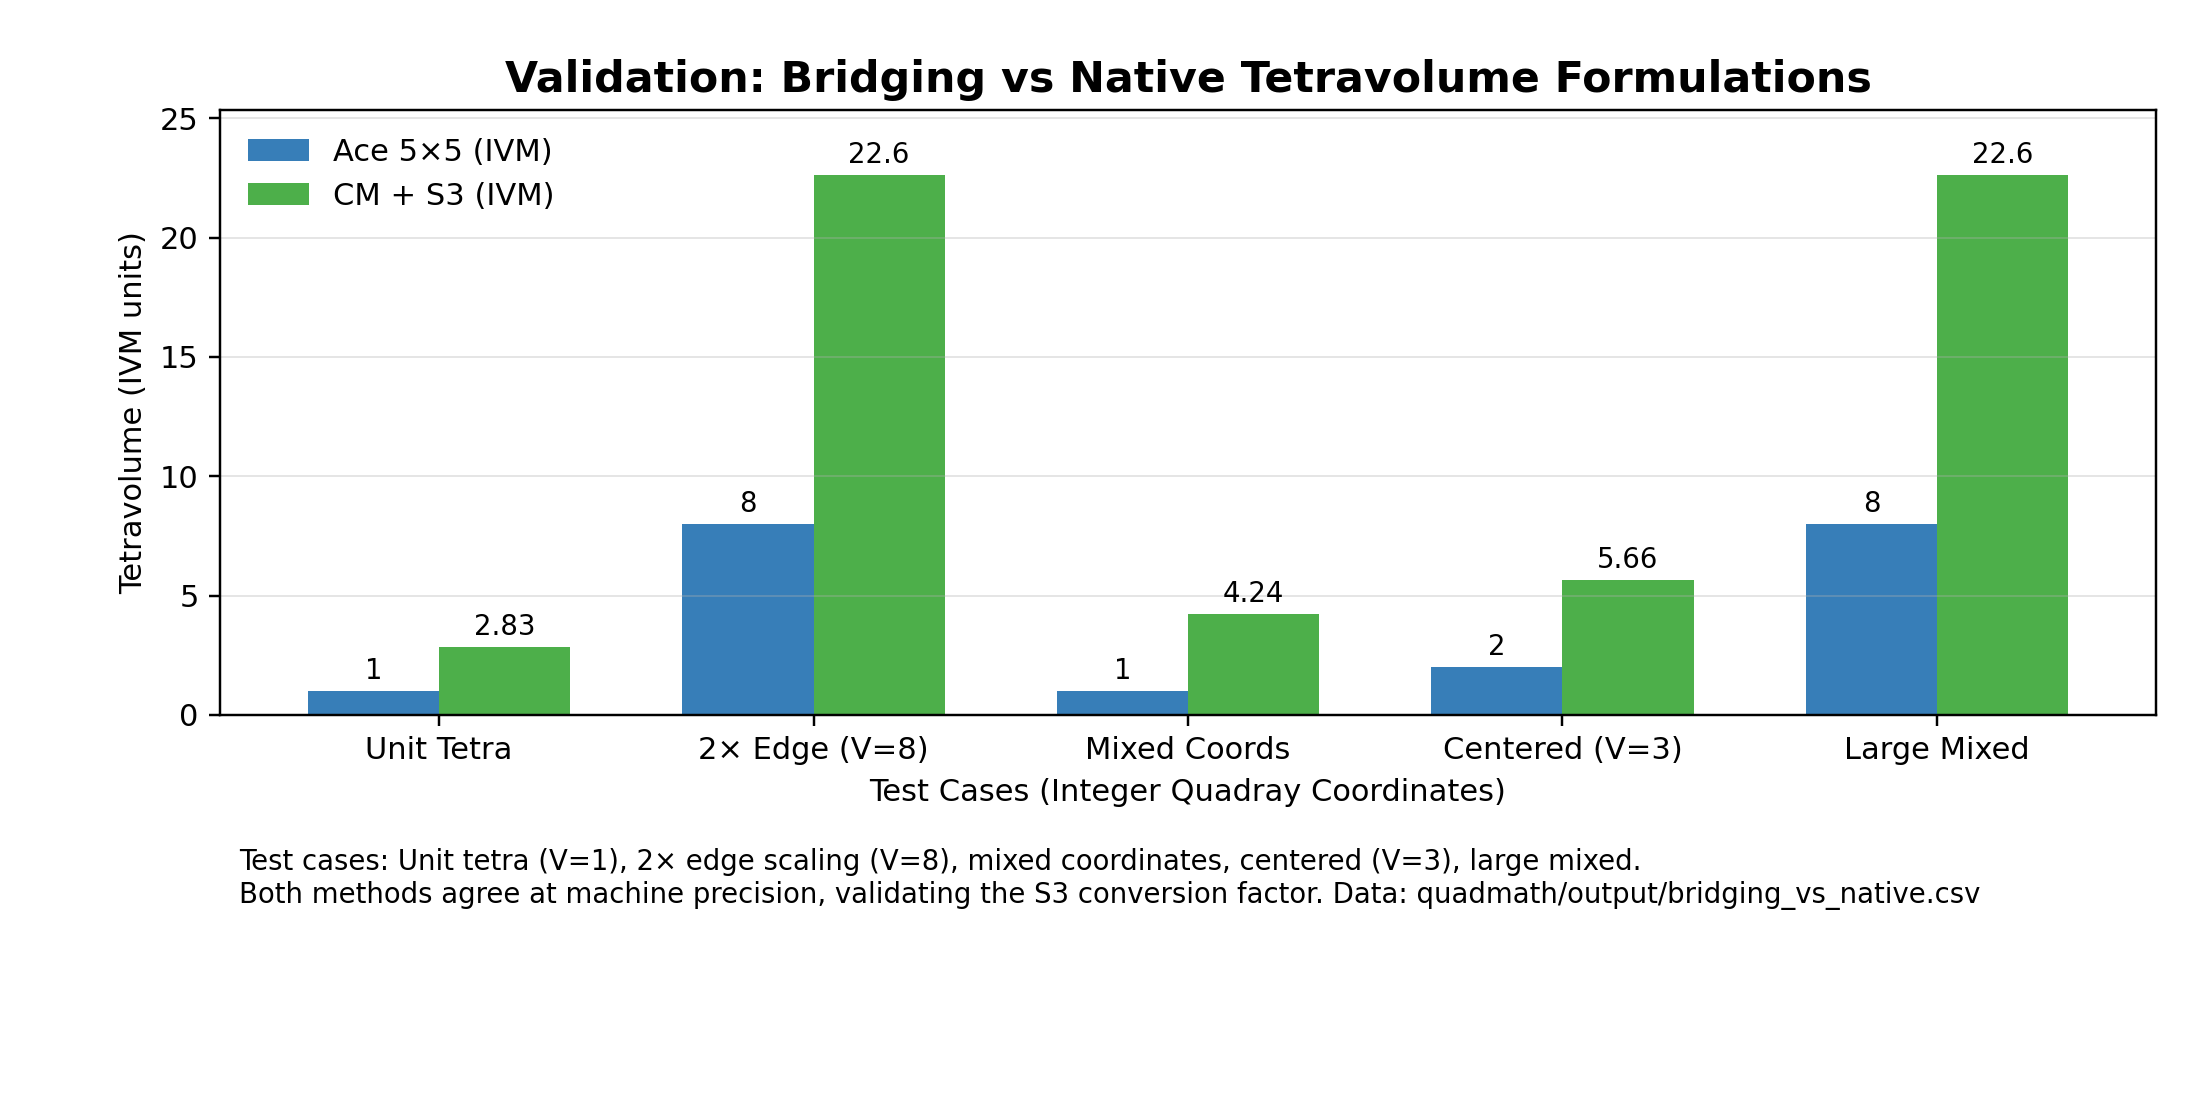
\includegraphics{../output/figures/bridging_vs_native.png}
\caption{\textbf{Validation of bridging vs native tetravolume
formulations across canonical examples}. This bar chart compares IVM
tetravolumes computed via two independent methods: the ``bridging''
approach using Cayley--Menger determinants on Euclidean edge lengths
converted to IVM units via the synergetics factor \(S3=\sqrt{9/8}\),
versus the ``native'' approach using Tom Ace's 5×5 determinant formula
that operates directly on Quadray coordinates without XYZ intermediates.
\textbf{Test cases}: Unit tetrahedron (V=1), 2× edge scaling (V=8),
mixed coordinate tetrahedron, centered tetrahedron (V=3), and large
mixed tetrahedron, all using integer Quadray coordinates.
\textbf{Results}: The overlapping bars demonstrate numerical agreement
at machine precision between the length-based Coxeter.4D approach
(Cayley--Menger + S3 conversion) and the coordinate-based Fuller.4D
approach (Ace 5×5), confirming the mathematical equivalence of these
formulations under synergetics unit conventions. Raw numerical data
saved as \passthrough{\lstinline!bridging\_vs\_native.csv!} for
reproducibility and further analysis.}
\end{figure}

\begin{figure}
\centering
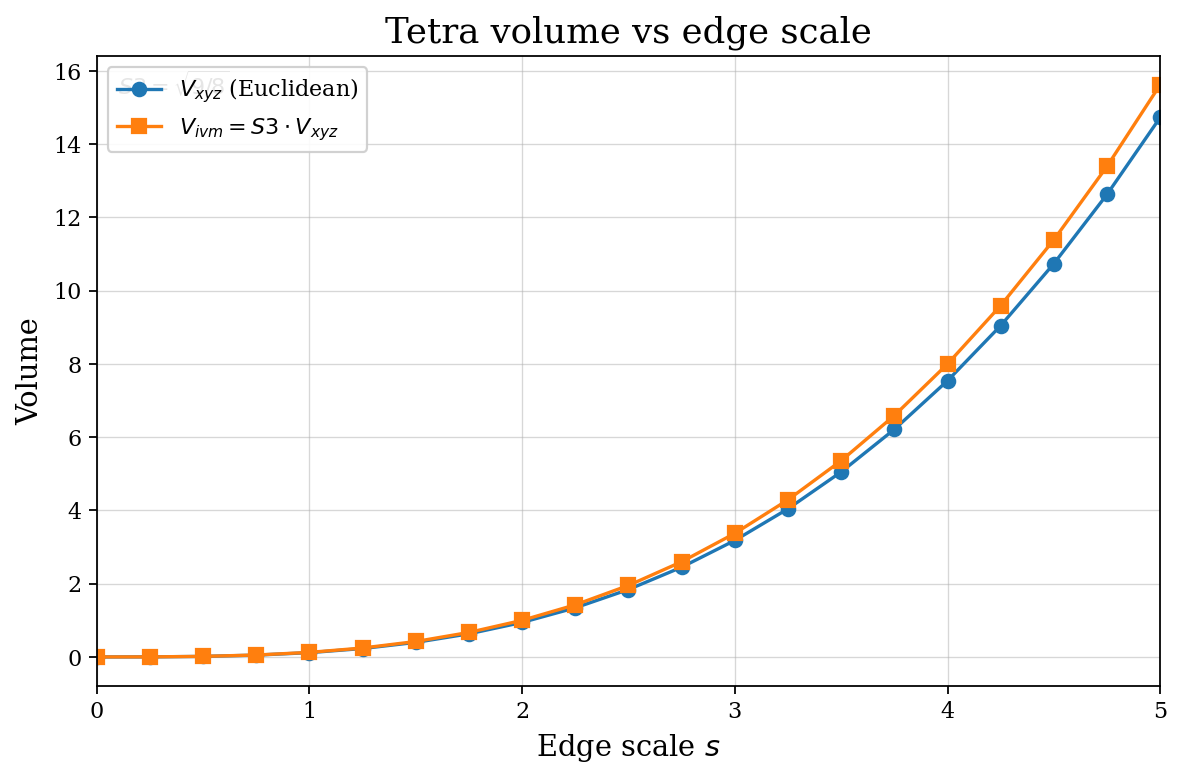
\includegraphics{../output/figures/volumes_scale_plot.png}
\caption{\textbf{Tetrahedron volume scaling relationships: Euclidean vs
IVM unit conventions}. This plot demonstrates the mathematical
relationship between edge length scaling and tetravolume under both
Euclidean (XYZ) and IVM (synergetics) unit conventions. \textbf{X-axis}:
Edge length scaling factor (0.5 to 2.0). \textbf{Y-axis}: Tetrahedron
volume in respective units. \textbf{Blue line (Euclidean)}: Volume
scales as the cube of edge length, following the standard
\(V = \frac{\sqrt{2}}{12} \cdot L^3\) relationship for regular
tetrahedra. \textbf{Orange line (IVM)}: Volume scales as the cube of
edge length but in IVM tetra-units, following
\(V_{ivm} = \frac{1}{8} \cdot L^3\) where the regular tetrahedron with
unit edge has volume 1/8. \textbf{Key insight}: The ratio between these
two scaling laws is the synergetics factor
\(S3 = \sqrt{9/8} \approx 1.06066\), which converts between Euclidean
and IVM volume conventions. \textbf{Mathematical foundation}: This
scaling relationship demonstrates how both conventions preserve the
cubic scaling relationship, but with different fundamental units
reflecting the different geometric assumptions of Coxeter.4D (Euclidean)
versus Fuller.4D (synergetics) frameworks. The plot provides the
theoretical foundation for understanding volume conversions and scaling
behavior in the IVM system.}
\end{figure}

\begin{figure}
\centering
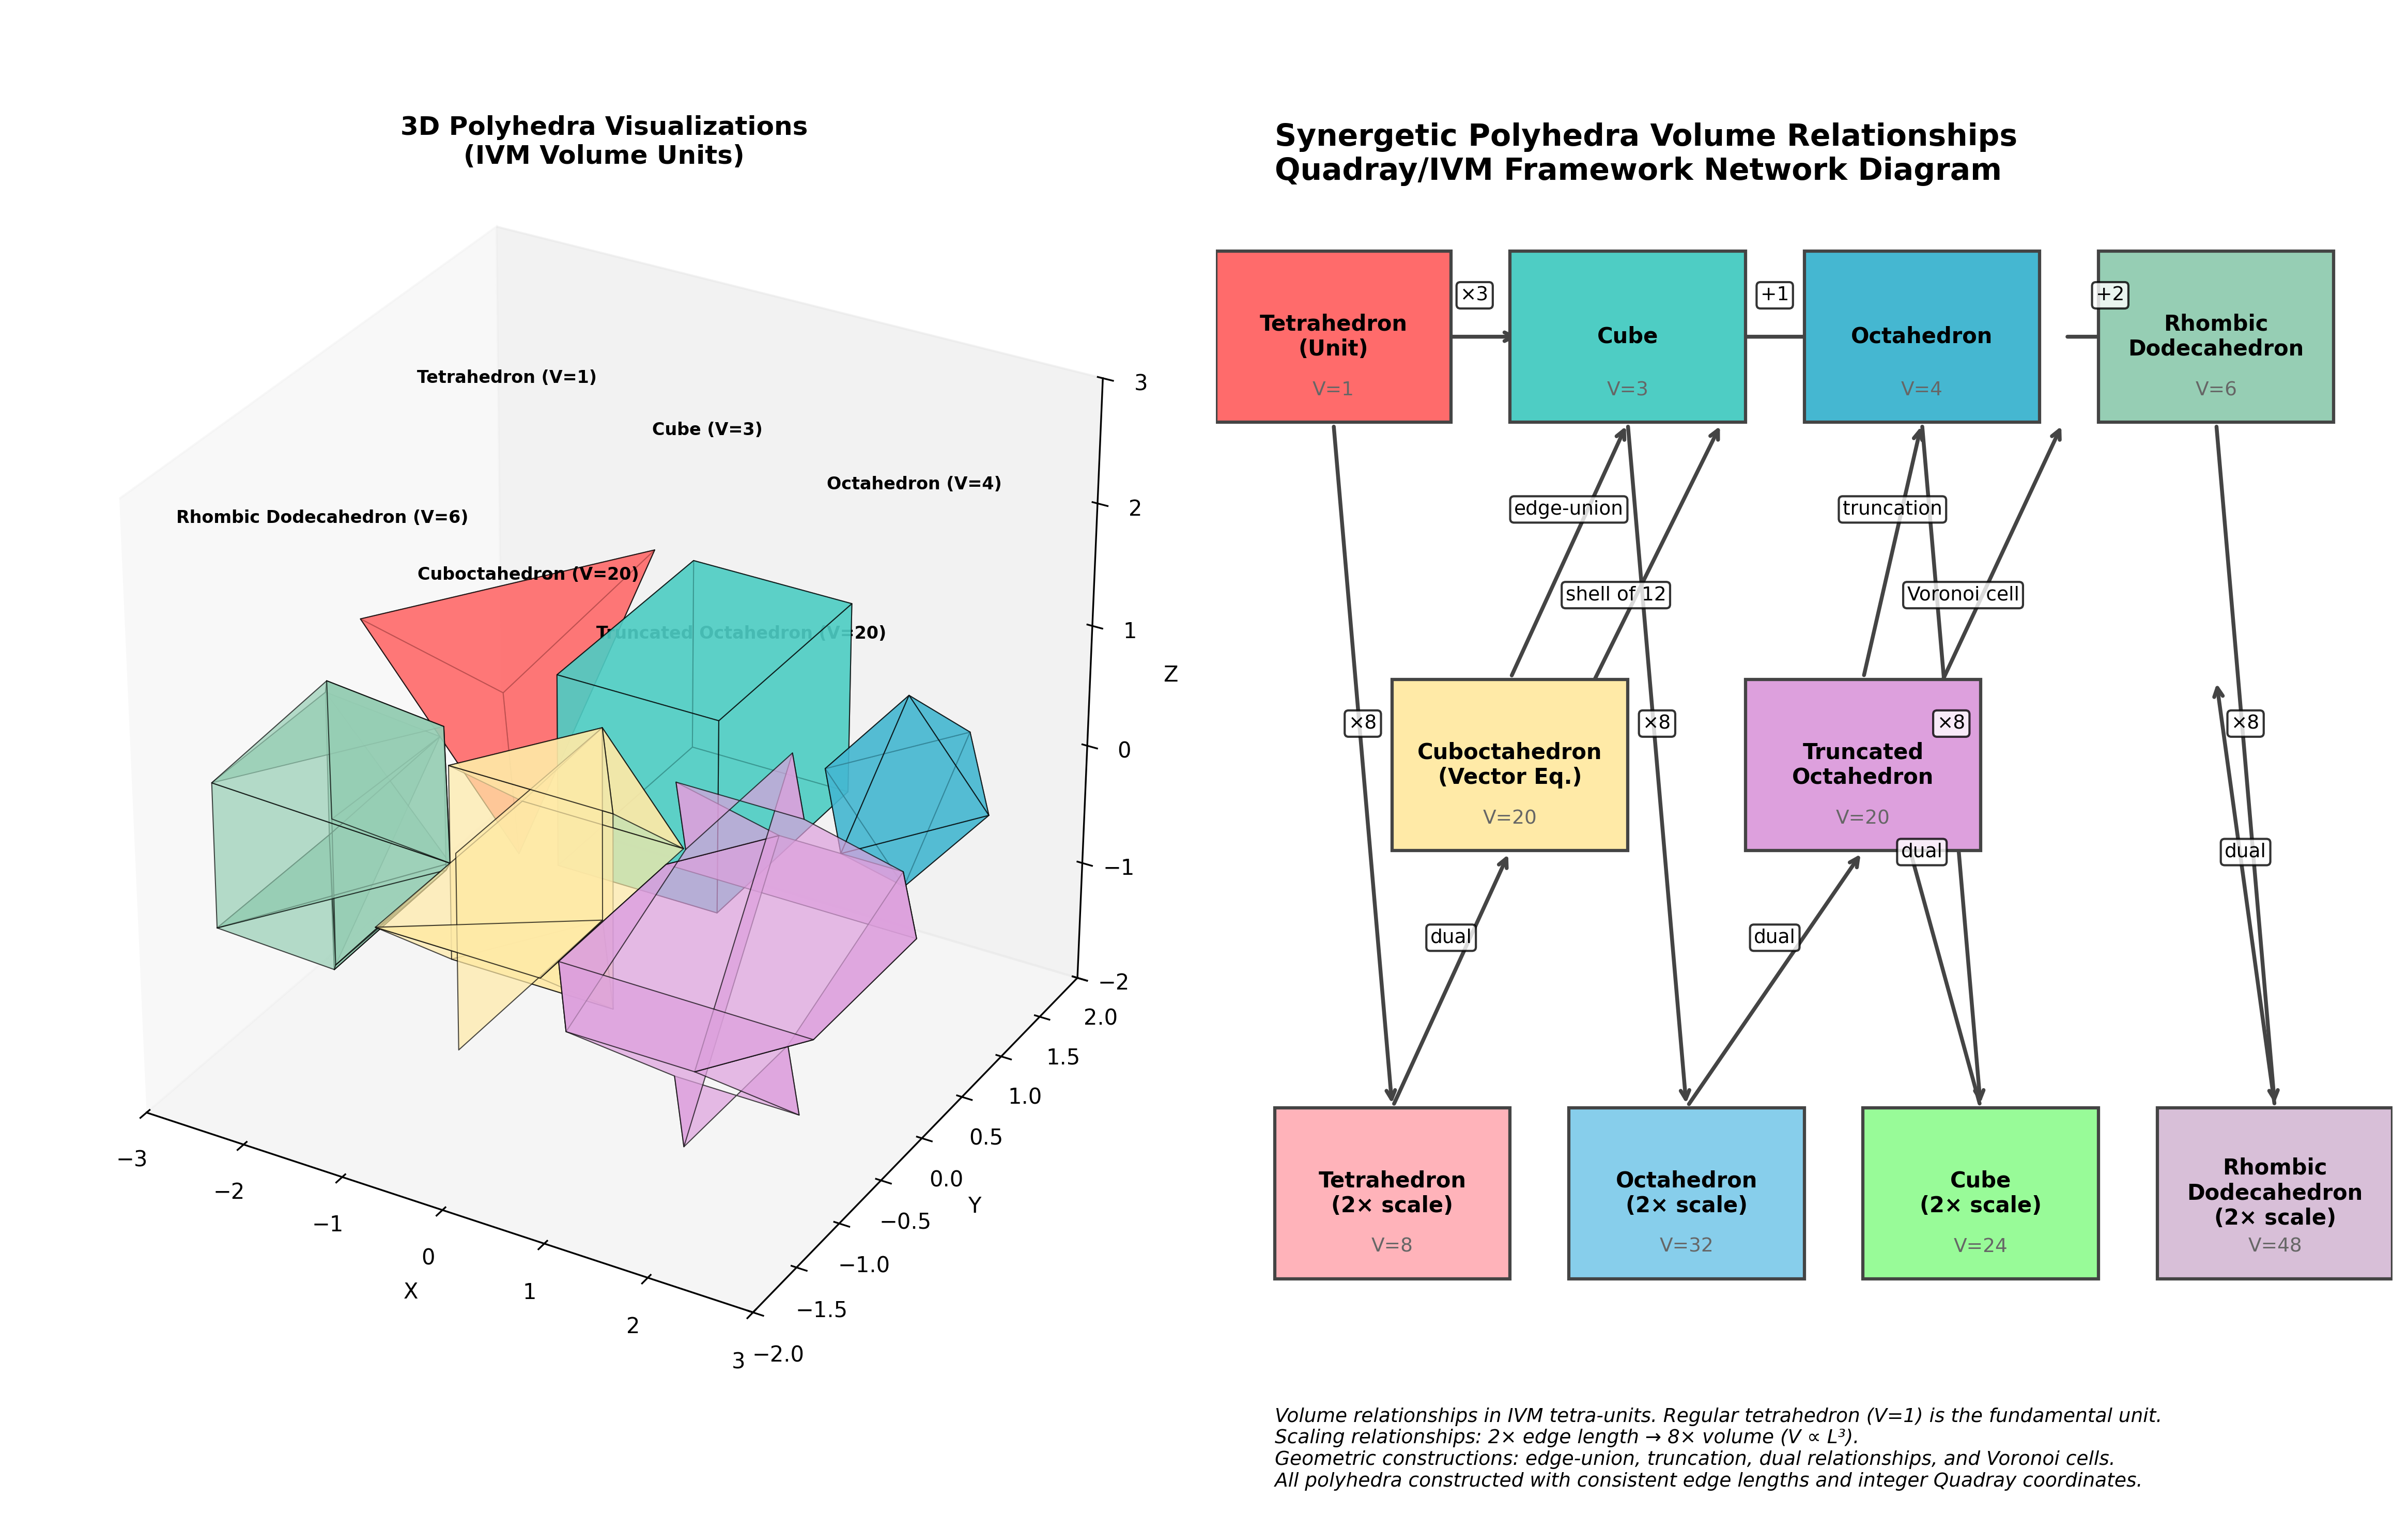
\includegraphics{../output/figures/polyhedra_quadray_constructions.png}
\caption{\textbf{Synergetic polyhedra volume relationships in the
Quadray/IVM framework (comprehensive visualization)}. This figure
combines 3D polyhedra visualizations with an extended network diagram
showing integer volume relationships among key synergetic polyhedra.
\textbf{Left panel (3D visualizations)}: Color-coded polyhedra including
regular tetrahedron (V=1, fundamental unit), cube (V=3), octahedron
(V=4), rhombic dodecahedron (V=6), cuboctahedron (V=20), and truncated
octahedron (V=20), all constructed with consistent edge lengths and
proper geometric faces. \textbf{Right panel (network diagram)}: Extended
volume relationships showing fundamental shapes (V=1,3,4,6), complex
constructions (V=20), and scaling relationships (2× edge length → 8×
volume). \textbf{Additional polyhedra}: Includes truncated octahedron
(V=20) and scaled variants demonstrating the ``third power'' volume
scaling law V ∝ L³ in IVM units. \textbf{Geometric constructions}:
Edge-union relationships, truncation operations, dual polyhedra, and
Voronoi cell constructions. \textbf{Fuller.4D significance}: These
integer volume ratios reflect the quantized nature of space-filling in
synergetics, where the regular tetrahedron provides a natural unit
container and other polyhedra emerge as integer multiples, supporting
discrete geometric computation and exact lattice-based optimization
methods. All constructions respect the IVM unit convention where the
regular tetrahedron has tetravolume 1.}
\end{figure}

\hypertarget{short-python-snippets}{%
\subsubsection{Short Python snippets}\label{short-python-snippets}}

\begin{lstlisting}[language=Python]
from quadray import Quadray, ace_tetravolume_5x5

o = Quadray(0,0,0,0)
p = Quadray(2,1,0,1)
q = Quadray(2,1,1,0)
r = Quadray(2,0,1,1)
assert ace_tetravolume_5x5(o,p,q,r) == 1  # unit IVM tetra
\end{lstlisting}

\begin{lstlisting}[language=Python]
import numpy as np
from cayley_menger import ivm_tetra_volume_cayley_menger

# Example: regular tetrahedron with edge length 1 (XYZ units)
d2 = np.ones((4,4)) - np.eye(4)  # squared distances
V_ivm = ivm_tetra_volume_cayley_menger(d2)   # = 1/8 in IVM tetra-units
\end{lstlisting}

\begin{lstlisting}[language=Python]
# SymPy implementation of Tom Ace 5×5 (symbolic determinant)
from sympy import Matrix

def qvolume(q0, q1, q2, q3):
    M = Matrix([
        q0 + (1,),
        q1 + (1,),
        q2 + (1,),
        q3 + (1,),
        [1, 1, 1, 1, 0],
    ])
    return abs(M.det()) / 4
\end{lstlisting}

\begin{lstlisting}[language=Python]
# Symbolic variant with SymPy (exact radicals)
from sympy import Matrix, sqrt, simplify
from symbolic import cayley_menger_volume_symbolic, convert_xyz_volume_to_ivm_symbolic

d2 = Matrix([[0,1,1,1],[1,0,1,1],[1,1,0,1],[1,1,1,0]])
V_xyz_sym = cayley_menger_volume_symbolic(d2)      # sqrt(2)/12
V_ivm_sym = simplify(convert_xyz_volume_to_ivm_symbolic(V_xyz_sym))  # 1/8
\end{lstlisting}

\hypertarget{random-tetrahedra-in-the-ivm-integer-volumes}{%
\subsubsection{Random tetrahedra in the IVM (integer
volumes)}\label{random-tetrahedra-in-the-ivm-integer-volumes}}

\begin{itemize}
\tightlist
\item
  The 12 CCP directions are the permutations of \((2,1,1,0)\). Random
  walks on this move set generate integer-coordinate Quadrays; resulting
  tetrahedra have integer tetravolumes.
\end{itemize}

\begin{lstlisting}[language=Python]
from itertools import permutations
from random import choice
from quadray import Quadray, ace_tetravolume_5x5

moves = [Quadray(*p) for p in set(permutations((2,1,1,0)))]

def random_walk(start: Quadray, steps: int) -> Quadray:
    cur = start
    for _ in range(steps):
        m = choice(moves)
        cur = Quadray(cur.a+m.a, cur.b+m.b, cur.c+m.c, cur.d+m.d)
    return cur

A = random_walk(Quadray(0,0,0,0), 1000)
B = random_walk(Quadray(0,0,0,0), 1000)
C = random_walk(Quadray(0,0,0,0), 1000)
D = random_walk(Quadray(0,0,0,0), 1000)
V = ace_tetravolume_5x5(A,B,C,D)            # integer
\end{lstlisting}

\hypertarget{algebraic-precision}{%
\subsubsection{Algebraic precision}\label{algebraic-precision}}

\begin{itemize}
\tightlist
\item
  Determinants via floating-point introduce rounding noise. For exact
  arithmetic, use the
  \href{https://en.wikipedia.org/wiki/Bareiss_algorithm}{Bareiss
  algorithm} (already used by
  \passthrough{\lstinline!ace\_tetravolume\_5x5!}) or symbolic engines
  (e.g., \passthrough{\lstinline!sympy!}). For large random-walk
  examples with integer inputs, volumes are exact integers.
\item
  When computing via XYZ determinants, high-precision floats (e.g.,
  \passthrough{\lstinline!gmpy2.mpfr!}) or symbolic matrices avoid
  vestigial errors; round at the end if the underlying result is known
  to be integral.
\end{itemize}

\hypertarget{xyz-determinant-and-the-s3-conversion}{%
\subsubsection{XYZ determinant and the S3
conversion}\label{xyz-determinant-and-the-s3-conversion}}

\begin{itemize}
\tightlist
\item
  Using XYZ coordinates of the four vertices: see Eq. \eqref{eq:xyz_det}
  for the determinant form and the S3 conversion to IVM units.
\end{itemize}

\hypertarget{d3-vs-r3-60-closing-the-lid-vs-orthogonal-cubing}{%
\subsubsection{D\^{}3 vs R\^{}3: 60° ``closing the lid'' vs orthogonal
``cubing''}\label{d3-vs-r3-60-closing-the-lid-vs-orthogonal-cubing}}

\begin{itemize}
\tightlist
\item
  \textbf{IVM (D\^{}3) heuristic}: From a 60--60--60 corner, three
  non-negative edge lengths \(A,B,C\) along quadray directions enclose a
  tetrahedron by ``closing the lid.'' In synergetics, the tetravolume
  scales as the simple product \(ABC\) under IVM conventions (unit
  regular tetra has volume 1). By contrast, in the orthogonal (R\^{}3)
  habit, one constructs a full parallelepiped (12 edges); the tetra
  occupies one-sixth of the triple product of edge vectors. The IVM path
  is more direct for tetrahedra.
\item
  \textbf{Pedagogical note}: Adopt a vector-first approach. Differences
  like \((P_i-P_0)\) denote edge vectors; Quadrays and Cartesian can be
  taught in parallel as vector languages on the same Euclidean
  container.
\end{itemize}

Reference notebook with worked examples and code: See the
\href{07_resources.md}{Resources} section for comprehensive educational
materials and computational implementations.

See implementation:
\passthrough{\lstinline!tetra\_volume\_cayley\_menger!}.

\begin{itemize}
\tightlist
\item
  Lattice projection: round to nearest integer quadray; renormalize to
  maintain non-negativity and a minimal zero.
\end{itemize}

\hypertarget{code-methods-anchors}{%
\subsection{Code methods (anchors)}\label{code-methods-anchors}}

\hypertarget{code:integer_tetra_volume}{%
\subsubsection{\texorpdfstring{\texttt{integer\_tetra\_volume}}{integer\_tetra\_volume}}\label{code:integer_tetra_volume}}

Source: \passthrough{\lstinline!src/quadray.py!} --- integer 3×3
determinant for lattice tetravolume.

\hypertarget{code:ace_tetravolume_5x5}{%
\subsubsection{\texorpdfstring{\texttt{ace\_tetravolume\_5x5}}{ace\_tetravolume\_5x5}}\label{code:ace_tetravolume_5x5}}

Source: \passthrough{\lstinline!src/quadray.py!} --- Tom Ace 5×5
determinant in IVM units.

\hypertarget{code:tetra_volume_cayley_menger}{%
\subsubsection{\texorpdfstring{\texttt{tetra\_volume\_cayley\_menger}}{tetra\_volume\_cayley\_menger}}\label{code:tetra_volume_cayley_menger}}

Source: \passthrough{\lstinline!src/cayley\_menger.py!} --- length-based
formula (XYZ units).

\hypertarget{code:ivm_tetra_volume_cayley_menger}{%
\subsubsection{\texorpdfstring{\texttt{ivm\_tetra\_volume\_cayley\_menger}}{ivm\_tetra\_volume\_cayley\_menger}}\label{code:ivm_tetra_volume_cayley_menger}}

Source: \passthrough{\lstinline!src/cayley\_menger.py!} ---
Cayley--Menger volume converted to IVM units.

\hypertarget{code:urner_embedding}{%
\subsubsection{\texorpdfstring{\texttt{urner\_embedding}}{urner\_embedding}}\label{code:urner_embedding}}

Source: \passthrough{\lstinline!src/conversions.py!} --- canonical XYZ
embedding.

\hypertarget{code:quadray_to_xyz}{%
\subsubsection{\texorpdfstring{\texttt{quadray\_to\_xyz}}{quadray\_to\_xyz}}\label{code:quadray_to_xyz}}

Source: \passthrough{\lstinline!src/conversions.py!} --- apply embedding
matrix to map Quadray to XYZ.

\hypertarget{code:bareiss_determinant_int}{%
\subsubsection{\texorpdfstring{\texttt{bareiss\_determinant\_int}}{bareiss\_determinant\_int}}\label{code:bareiss_determinant_int}}

Source: \passthrough{\lstinline!src/linalg\_utils.py!} --- exact integer
Bareiss determinant.

\hypertarget{information-geometry-methods-anchors}{%
\subsubsection{Information geometry methods
(anchors)}\label{information-geometry-methods-anchors}}

\hypertarget{code:fisher_information_matrix}{%
\paragraph{\texorpdfstring{\texttt{fisher\_information\_matrix}}{fisher\_information\_matrix}}\label{code:fisher_information_matrix}}

Source: \passthrough{\lstinline!src/information.py!} --- empirical
outer-product estimator.

\hypertarget{code:natural_gradient_step}{%
\paragraph{\texorpdfstring{\texttt{natural\_gradient\_step}}{natural\_gradient\_step}}\label{code:natural_gradient_step}}

Source: \passthrough{\lstinline!src/information.py!} --- damped
inverse-Fisher step.

\hypertarget{code:free_energy}{%
\paragraph{\texorpdfstring{\texttt{free\_energy}}{free\_energy}}\label{code:free_energy}}

Source: \passthrough{\lstinline!src/information.py!} --- discrete-state
variational free energy.

\hypertarget{code:discrete_ivm_descent}{%
\paragraph{\texorpdfstring{\texttt{discrete\_ivm\_descent}}{discrete\_ivm\_descent}}\label{code:discrete_ivm_descent}}

Source: \passthrough{\lstinline!src/discrete\_variational.py!} ---
greedy integer-valued descent over the IVM using canonical neighbor
moves; returns a
\passthrough{\lstinline!DiscretePath with visited Quadrays and objective values. Pairs with!}animate\_discrete\_path`.

\hypertarget{code:animate_discrete_path}{%
\paragraph{\texorpdfstring{\texttt{animate\_discrete\_path}}{animate\_discrete\_path}}\label{code:animate_discrete_path}}

Source: \passthrough{\lstinline!src/visualize.py!} --- animate a
\passthrough{\lstinline!DiscretePath!} to MP4; saves CSV/NPZ trajectory
to \passthrough{\lstinline!quadmath/output/!}.

Relevant tests (\passthrough{\lstinline!tests/!}):

\begin{itemize}
\tightlist
\item
  \passthrough{\lstinline!test\_quadray.py!} (unit IVM tetra,
  divisibility-by-4 scaling, Ace vs.~integer method)
\item
  \passthrough{\lstinline!test\_quadray\_cov.py!} (Ace determinant basic
  check)
\item
  \passthrough{\lstinline!test\_cayley\_menger.py!} (regular tetra
  volume in XYZ units)
\item
  \passthrough{\lstinline!test\_linalg\_utils.py!} (Bareiss determinant
  behavior)
\item
  \passthrough{\lstinline!test\_examples.py!},
  \passthrough{\lstinline!test\_examples\_cov.py!} (neighbors, examples)
\item
  \passthrough{\lstinline!test\_metrics.py!},
  \passthrough{\lstinline!test\_metrics\_cov.py!},
  \passthrough{\lstinline!test\_information.py!},
  \passthrough{\lstinline!test\_paths.py!},
  \passthrough{\lstinline!test\_paths\_cov.py!}
\end{itemize}

\hypertarget{reproducibility-checklist}{%
\subsection{Reproducibility checklist}\label{reproducibility-checklist}}

\begin{itemize}
\tightlist
\item
  All formulas used in the paper are implemented in
  \passthrough{\lstinline!src/!} and verified by
  \passthrough{\lstinline!tests/!}.
\item
  Determinants are computed with exact arithmetic for integer inputs;
  floating-point paths are used only where appropriate and results are
  converted (e.g., via S3) as specified.
\item
  Random-walk experiments produce integer volumes; Ace 5×5 determinant
  agrees with length-based methods.
\item
  Volume tracking: monitor integer simplex volume to detect convergence
  plateaus.
\item
  Face/edge analyses: interpret sensitivity along edges; subspace
  searches across faces.
\end{itemize}

\end{document}
